\chapter{Inflación impulsada por un campo escalar rodante}

\lectureoverview{Una pregunta pendiente de la clase anterior proporciona la ecuación que organiza esta exposición,
\(\ddot\phi+3H\dot\phi=-V'(\phi)\): ¿qué se mueve, qué ejerce la fuerza y por qué la expansión se parece a la fricción? Primero derivamos la ecuación en una caja fija y después en una caja en expansión. Al acoplarla a la ecuación de Friedmann obtenemos el mecanismo de rodadura lenta, en el que un potencial escalar alto y poco inclinado impulsa una expansión casi exponencial. La inflación diluye los monopolos y alisa la geometría; al terminar, recalienta el universo y da comienzo al Big Bang caliente convencional. Entonces surge inevitablemente la última pregunta: si la inflación alisa con tanta eficacia, ¿de dónde salió la estructura? Un cálculo unidimensional de una cáustica muestra cómo pequeñas variaciones de velocidad crean láminas, filamentos y nudos, mientras deja para la próxima clase el origen cuántico de esas variaciones.}

\section{¿Qué actúa sobre qué?}

La pregunta inicial recuerda la ecuación
\begin{equation}
\ddot\phi+3H\dot\phi
=F(\phi)
=-\frac{dV}{d\phi}
\label{eq:c09-opening}
\end{equation}
y pregunta qué tipo de fuerza \(F\) puede actuar sobre un campo. No es una cuestión secundaria. Para responderla debemos reconstruir la mecánica del campo, y al hacerlo comenzamos a estudiar la inflación misma.

Un campo escalar asigna un número \(\phi(\mathbf x,t)\) a cada punto del espacio y del tiempo. Los campos eléctrico y magnético transportan energía; un campo escalar también puede hacerlo. El campo que necesitamos aquí es hipotético: no se ha identificado experimentalmente ningún inflatón concreto, así que se desconoce su energía en función del valor del campo. Por eso lo representamos mediante una densidad de energía potencial no especificada
\begin{equation}
V=V(\phi).
\label{eq:c09-potential}
\end{equation}
Distintos valores de \(\phi\) corresponden a distintas cantidades de energía almacenada por unidad de volumen físico.

No hay razón para que \(\phi=0\) tenga energía nula. El origen del espacio de campos es una convención, sobre todo en el caso de un campo aún no descubierto, y un cambio en la coordenada usada para etiquetar los valores del campo no tiene por qué situar en el origen el mínimo de \(V\). La gráfica de \(V(\phi)\) describe pendientes y alturas relativas, no un punto de partida privilegiado para el campo.

La energía potencial es la parte que queda cuando el campo está momentáneamente estático. Si el campo cambia con el tiempo, también tiene energía cinética. La cantidad \(\dot\phi\) no es la velocidad de un objeto que se desplaza por el espacio ordinario; es la tasa de cambio del valor del campo, una velocidad en el espacio de campos. Una cuerda elástica ofrece una analogía útil. Su desplazamiento es un campo definido sobre un mundo unidimensional, y un elemento vibrante de la cuerda tiene energía cinética proporcional al cuadrado de su derivada temporal.

El coeficiente de ese cuadrado se puede absorber en la definición del campo. Si se parte de
\begin{equation}
\frac12 n^2\dot\phi^{\,2},
\end{equation}
el cambio de variable
\begin{equation}
\chi=n\phi
\end{equation}
convierte el término en \(\dot\chi^{\,2}/2\). Por tanto, podemos elegir un campo con normalización canónica y escribir, en la aproximación homogénea,
\begin{equation}
\rho_\phi=\frac12\dot\phi^{\,2}+V(\phi).
\label{eq:c09-rho-homogeneous}
\end{equation}
Esta elección normaliza la coordenada en el espacio de campos; no afirma que la masa literal de una partícula se haya fijado en uno.

\section{Mecánica en una caja fija}

Consideremos una caja pequeña en la que el campo sea casi constante en todo el espacio. Su densidad de energía tiene la misma forma matemática que la energía de una partícula de masa unitaria: energía cinética más potencial. La densidad lagrangiana correspondiente lleva el signo opuesto para el potencial,
\begin{equation}
\mathcal L_\phi
=\frac12\dot\phi^{\,2}-V(\phi).
\label{eq:c09-lagrangian-density}
\end{equation}
La analogía es matemática. La coordenada generalizada es el valor del campo, no la posición espacial de una partícula.

La ecuación de Euler--Lagrange es
\begin{equation}
\frac{d}{dt}
\left(
\frac{\partial\mathcal L_\phi}{\partial\dot\phi}
\right)
=
\frac{\partial\mathcal L_\phi}{\partial\phi}.
\label{eq:c09-el-fixed}
\end{equation}
Aquí la variable de velocidad es \(\dot\phi\), así que
\begin{equation}
\frac{\partial\mathcal L_\phi}{\partial\dot\phi}=\dot\phi,
\qquad
\frac{\partial\mathcal L_\phi}{\partial\phi}=-V'(\phi),
\end{equation}
y obtenemos
\begin{equation}
\ddot\phi=-V'(\phi)\equiv F(\phi).
\label{eq:c09-fixed-eom}
\end{equation}
La segunda derivada es la aceleración de la coordenada del campo, y la pendiente negativa del potencial es su fuerza.

\begin{figure}[htbp]
\centering
\includegraphics[width=0.88\textwidth]{lecture_09_figure_03.png}
\caption{La parte legible de la pizarra muestra \(V(\phi)\) en la ecuación para la caja fija \(\ddot\phi=-\partial V/\partial\phi\). La expresión de Euler--Lagrange de la parte superior está parcialmente recortada y tapada, así que la ecuación ~\eqref{eq:c09-el-fixed} se reconstruye a partir de la derivación, en lugar de citarse como una transcripción completa de la pizarra.}
\label{fig:c09-fixed-board}
\lectureframe{00:10:53.836}
\end{figure}

\begin{classroomqa}
\audiencequestion{¿Qué es la fuerza y sobre qué actúa?}
\lecturerresponse{El objeto que evoluciona es el valor escalar \(\phi\). La cantidad \(-V'(\phi)\) es una fuerza en el espacio de campos: acelera el valor del campo hacia valores menores de la energía potencial, del mismo modo que \(-dV/dx\) acelera la coordenada de una partícula. No es una nueva fuerza vectorial que empuje un cuerpo material por el espacio ordinario. \lecturetimestamp{00:00:27--00:00:49; 00:10:41--00:11:29}}
\end{classroomqa}

El campo completo puede depender del espacio. Para un escalar canónico en una geometría en expansión espacialmente plana, su densidad de energía local contiene
\begin{equation}
\rho_\phi
=
\frac12\dot\phi^{\,2}
+\frac{1}{2a^2}\lvert\nabla\phi\rvert^2
+V(\phi).
\label{eq:c09-rho-full}
\end{equation}
Omitimos el término de gradiente porque la expansión estira las variaciones hasta longitudes de onda grandes, de modo que el campo es casi uniforme dentro de la caja pequeña. Es una aproximación justificada por el contexto cosmológico, no una negación de que puedan existir ondas escalares o fluctuaciones espaciales.

\section{La caja en expansión}

La primera derivación responde a la pregunta inicial, pero aún no es la derivación cosmológica. Las ecuaciones ~\eqref{eq:c09-rho-homogeneous} y \eqref{eq:c09-lagrangian-density} son densidades. El volumen físico de una caja comóvil unitaria es proporcional a \(a^3(t)\), por lo que su lagrangiano es
\begin{equation}
L_\phi
=a^3(t)
\left[
\frac12\dot\phi^{\,2}-V(\phi)
\right].
\label{eq:c09-comoving-lagrangian}
\end{equation}
En una caja estática, el factor \(a^3\) sería irrelevante. En cosmología depende del tiempo, y esa dependencia aporta el término que faltaba.

\begin{figure}[htbp]
\centering
\includegraphics[width=0.88\textwidth]{lecture_09_figure_04.png}
\caption{A la izquierda se ve una curva de potencial dibujada a mano, mientras que a la derecha aparecen fragmentos de las expresiones de energía y del lagrangiano. La curva y el cambio de signo se distinguen con claridad; el desarrollo algebraico completo de la ecuación ~\eqref{eq:c09-comoving-lagrangian} procede de la explicación oral, porque el profesor tapa parte de la pizarra.}
\label{fig:c09-potential-board}
\lectureframe{00:13:26.528}
\end{figure}

Al aplicar la ecuación de Euler--Lagrange a \(L_\phi\) se obtiene
\begin{align}
\frac{d}{dt}\left(a^3\dot\phi\right)
&=-a^3V'(\phi), \label{eq:c09-a3-form}\\
a^3\ddot\phi+3a^2\dot a\,\dot\phi
&=-a^3V'(\phi),\\
\ddot\phi+3\frac{\dot a}{a}\dot\phi
&=-V'(\phi).
\end{align}
Con \(H=\dot a/a\), el resultado es
\begin{equation}
\boxed{\ddot\phi+3H\dot\phi=-V'(\phi)}.
\label{eq:c09-hubble-friction}
\end{equation}
La ecuación que recordamos al principio ya está derivada, no solo evocada.

\begin{figure}[htbp]
\centering
\includegraphics[width=0.96\textwidth]{lecture_09_figure_05.png}
\caption{Dinámica en la caja fija a la izquierda y corrección debida a la expansión de la caja a la derecha. La pizarra visible respalda la secuencia desde \(d(a^3\dot\phi)/dt\) hasta las formas \(3\dot a/a\) y \(3H\); los miembros derechos recortados se completan con la ecuación ~\eqref{eq:c09-a3-form}.}
\label{fig:c09-expanding-board}
\lectureframe{00:18:35.380}
\end{figure}

\begin{classroomqa}
\audiencequestion{¿Se puede visualizar de forma más concreta la fuerza \(F\)?}
\lecturerresponse{Representemos \(V(\phi)\) como un paisaje cuya coordenada horizontal sea el valor del campo. La pendiente determina la fuerza, \(F=-V'(\phi)\). Una pendiente descendente pronunciada produce un impulso grande en el espacio de campos; una pendiente suave, uno pequeño. La imagen ayuda a representar la coordenada unidimensional del campo, pero no es una colina literal situada en el espacio físico. \lecturetimestamp{00:18:26--00:19:18}}
\end{classroomqa}

\section{Fricción de Hubble y movimiento terminal}

Pasemos el término central de la ecuación ~\eqref{eq:c09-hubble-friction} al miembro derecho:
\begin{equation}
\ddot\phi=-V'(\phi)-3H\dot\phi.
\end{equation}
En un universo en expansión, \(H>0\), el segundo término siempre se opone a la velocidad del campo. Por tanto, se comporta como una fuerza viscosa. Una roca soltada en miel espesa acelera al principio, pero la resistencia aumenta con la velocidad hasta que alcanza una velocidad terminal. La mnemotecnia \emph{\(H\) para miel } recoge la analogía, mientras que la ecuación expresa su contenido real. Si \(H\) cambia con el tiempo cósmico, también cambia la viscosidad efectiva, igual que la viscosidad ordinaria cambia con la temperatura.

Cuando la fricción domina sobre la inercia, \(\lvert\ddot\phi\rvert\ll3H\lvert\dot\phi\rvert\), y el campo se aproxima rápidamente a
\begin{equation}
3H\dot\phi\simeq -V'(\phi),
\qquad
\dot\phi\simeq-\frac{V'(\phi)}{3H}.
\label{eq:c09-terminal}
\end{equation}
Un potencial poco inclinado proporciona una fuerza pequeña, mientras que un \(H\) grande produce una resistencia intensa. Ambos efectos hacen que \(\dot\phi\) sea pequeño y suelen hacer que la densidad cinética \(\dot\phi^2/2\) sea pequeña en comparación con \(V\).

\begin{classroomqa}
\audiencequestion{¿Esta derivación se basa en el principio de mínima acción?}
\lecturerresponse{Sí. La ecuación ~\eqref{eq:c09-hubble-friction} se obtiene extremando la acción construida a partir de la ecuación ~\eqref{eq:c09-comoving-lagrangian}. También se puede tomar la ecuación del campo como ley dinámica de partida, pero la derivación variacional explica exactamente por qué el volumen en expansión aporta \(3H\dot\phi\). \lecturetimestamp{00:25:40--00:26:15}}
\end{classroomqa}

\begin{classroomqa}
\audiencequestion{Si el nuevo término actúa como fricción, ¿adónde va la energía perdida?}
\lecturerresponse{Una roca real en la miel transfiere energía mecánica a calor. La afirmación cosmológica es más sutil. El lagrangiano de la caja comóvil depende explícitamente del tiempo a través de \(a(t)\), así que la energía mecánica ordinaria de esa caja no se conserva por simetría ante traslaciones temporales. La conservación local covariante del tensor de energía-momento sí se cumple:
\[
\dot\rho_\phi+3H(\rho_\phi+p_\phi)=0,
\qquad
p_\phi=\frac12\dot\phi^{\,2}-V(\phi).
\]
Para un escalar homogéneo, esto se convierte en \(\dot\rho_\phi=-3H\dot\phi^{\,2}\): el campo realiza trabajo sobre la geometría en expansión. Lo que falla es la idea ingenua de una energía global conservada para el universo en evolución, no la conservación local del tensor de energía-momento. \lecturetimestamp{00:26:16--00:27:57}}
\end{classroomqa}

\section{El campo impulsa la expansión}

Hasta ahora, la expansión ha actuado sobre el escalar. Eso es solo la mitad del ciclo de retroalimentación. La densidad de energía del escalar también determina la expansión mediante la ecuación de Friedmann en un espacio plano,
\begin{equation}
H^2=\left(\frac{\dot a}{a}\right)^2
=\frac{8\pi G}{3}\rho.
\label{eq:c09-friedmann}
\end{equation}
Para un escalar casi homogéneo,
\begin{equation}
H^2
=\frac{8\pi G}{3}
\left[
\frac12\dot\phi^{\,2}+V(\phi)
\right].
\label{eq:c09-friedmann-scalar}
\end{equation}
La expansión amortigua el campo, y el campo amortiguado puede, a su vez, mantener la densidad de energía que impulsa la expansión.

\begin{classroomqa}
\audiencequestion{¿Este escalar hipotético es lo que se llama inflatón?}
\lecturerresponse{Sí. El nombre describe el papel que se le atribuye: un campo escalar cuya energía potencial casi constante impulsa la inflación. Darle nombre al campo no identifica su física de partículas. El inflatón concreto, sus acoplamientos e incluso la posibilidad de que este papel lo desempeñara un solo escalar elemental dependen del modelo. \lecturetimestamp{00:30:26--00:31:28}}
\end{classroomqa}

\begin{classroomqa}
\audiencequestion{¿Hay pruebas experimentales del inflatón?}
\lecturerresponse{No se ha detectado directamente en el laboratorio ningún campo inflatón concreto. Las pruebas son indirectas: la dinámica inflacionaria ofrece un marco satisfactorio para explicar la planitud observada y las perturbaciones primordiales, pero muchos potenciales pueden ajustarse a esos hechos generales. Este apoyo indirecto debe distinguirse del conocimiento de la implementación microscópica. \lecturetimestamp{00:31:29--00:33:02}}
\end{classroomqa}

\begin{classroomqa}
\audiencequestion{¿Todos los campos transportan energía, y una excitación escalar sería un bosón?}
\lecturerresponse{Los campos físicos contribuyen a la energía y al momento. Al cuantizar un campo escalar se obtienen cuantos bosónicos de espín cero. El fondo clásico homogéneo que se usa en inflación no se representa mejor como una partícula ordinaria, aunque, después de la inflación, sus oscilaciones pueden describirse en términos de cuantos de inflatón. \lecturetimestamp{00:33:03--00:35:20}}
\end{classroomqa}

\begin{classroomqa}
\audiencequestion{¿Podría el campo de Higgs ser el inflatón?}
\lecturerresponse{Se necesita un escalar, así que la analogía es natural, pero el Higgs observado, con su potencial y sus acoplamientos ordinarios del Modelo Estándar, no es automáticamente el campo descrito por esta meseta sencilla. Los modelos de inflación de Higgs añaden estructura gravitatoria no mínima. Nada de lo expuesto aquí identifica el inflatón con el Higgs. \lecturetimestamp{00:35:21--00:37:11}}
\end{classroomqa}

Imaginemos ahora que \(V(\phi)\) es grande, pero varía suavemente a lo largo de un intervalo extenso. La ecuación ~\eqref{eq:c09-terminal} mantiene el campo en movimiento lento y, por tanto,
\begin{equation}
\frac12\dot\phi^{\,2}\ll V(\phi).
\end{equation}
La ecuación de Friedmann se reduce a
\begin{equation}
H^2\simeq\frac{8\pi G}{3}V(\phi),
\qquad
H\simeq
\sqrt{\frac{8\pi G}{3}V(\phi)}.
\label{eq:c09-potential-dominated}
\end{equation}
La derivada \(V'(\phi)\) controla el movimiento lento del campo; la altura \(V(\phi)\) controla la rápida expansión del espacio.

\begin{figure}[htbp]
\centering
\includegraphics[width=0.92\textwidth]{lecture_09_figure_06.png}
\caption{La ecuación de Friedmann, la densidad de energía escalar y la expresión encuadrada dominada por el potencial. El término de raíz cuadrada de \(V(\phi)\) se distingue con claridad; el \(H\simeq\) inicial de la ecuación ~\eqref{eq:c09-potential-dominated} es la forma completa estándar, respaldada por la explicación oral.}
\label{fig:c09-friedmann-board}
\lectureframe{00:41:04.178}
\end{figure}

Si \(V\) cambia solo ligeramente mientras el campo recorre la meseta, entonces \(H\) es casi constante. Al integrar \(\dot a/a\simeq H\) se obtiene
\begin{equation}
a(t)\simeq a_i e^{H(t-t_i)}.
\label{eq:c09-exponential}
\end{equation}
Esto es inflación. Un tiempo de duplicación aproximado de \(10^{-32}\,\mathrm{s}\) en el universo temprano da una idea de su intensidad; el número es ilustrativo y depende de la escala de energía de la inflación.

\begin{classroomqa}
\audiencequestion{¿Cómo puede un campo que se mueve lentamente producir un universo que se expande con rapidez?}
\lecturerresponse{Lo que se mueve lentamente es \(\phi\), no \(a\). La fricción de Hubble impide que el campo se precipite por el potencial, de modo que \(V(\phi)\) permanece casi constante. Un \(V\) grande y casi constante da un \(H\) grande y casi constante, y entonces el factor de escala crece exponencialmente. La pequeña pendiente controla el movimiento del campo; la meseta alta controla la expansión cósmica. \lecturetimestamp{00:40:06--00:41:39}}
\end{classroomqa}

\section{¿Por qué introducir la inflación?}

Alan Guth propuso la inflación alrededor de 1980 para resolver problemas cosmológicos concretos. Los trabajos posteriores, en particular los de Andrei Linde y otros, desarrollaron versiones en las que la fase inflacionaria termina de forma gradual. El marco general concuerda con observaciones importantes, pero no se ha establecido un potencial único; el éxito del mecanismo no debe confundirse con que cada detalle esté confirmado experimentalmente.

\subsection{El problema de los monopolos}

Las teorías de gran unificación suelen permitir monopolos magnéticos. Según una estimación aproximada, serían extraordinariamente pesados, quizá con una masa muchas veces superior a la del protón; la masa precisa depende de la teoría y no tiene por qué ser exactamente la masa de Planck. Un universo temprano lo bastante caliente produciría pares de monopolo--antimonopolo. La carga magnética protegería entonces una población relicta a medida que el universo se enfriara.

No se observa una densidad relicta sustancial. En particular, las cargas magnéticas que se moviesen libremente drenarían con eficacia los campos magnéticos galácticos, del mismo modo que las cargas eléctricas móviles apantallan o descargan los campos eléctricos. La persistencia del magnetismo galáctico impone, por tanto, límites estrictos a los monopolos cósmicos. La inflación resuelve el problema al aumentar enormemente el volumen: los monopolos que hubiera antes de la inflación se diluyen hasta que prácticamente ninguno queda en nuestra región observable.

\subsection{Uniformidad y planitud}

La radiación cósmica de fondo es extraordinariamente uniforme. Sin inflación, en la extrapolación más sencilla del Big Bang caliente, las regiones muy separadas de la superficie de última dispersión habrían tenido muy poco contacto causal ordinario para explicar que sus temperaturas coincidan tanto. La inflación parte de una región mucho menor, conectada causalmente, y la estira hasta abarcar el universo observable. También hace que la curvatura espacial tienda a cero, de manera muy parecida a como una pequeña región de una esfera enormemente inflada parece plana.

La cantidad de expansión se mide mediante el número de pliegues \(e\),
\begin{equation}
N\equiv \ln\frac{a_{\rm end}}{a_{\rm start}}
=\int_{t_{\rm start}}^{t_{\rm end}}H\,dt.
\label{eq:c09-efolds}
\end{equation}
Usaremos \(N\gtrsim60\) como límite inferior útil de orden de magnitud. El requisito exacto depende de la escala inflacionaria y de la historia del recalentamiento; distintos modelos dan estimaciones en el amplio intervalo cercano a \(40\)--\(80\). Un mayor desorden inicial o una densidad indeseada de reliquias pueden exigir más inflación.

\begin{classroomqa}
\audiencequestion{Si el universo inicial fuera completamente caótico, ¿bastarían aun así sesenta pliegues de \(e\)?}
\lecturerresponse{No necesariamente. Sesenta es una estimación convencional del límite inferior para resolver los problemas estándar del horizonte y la planitud, bajo ciertos supuestos. Un estado inicial más irregular puede exigir una meseta lisa más larga. No se afirma que un único número universal borre cualquier condición inicial concebible. \lecturetimestamp{00:55:23--00:56:48}}
\end{classroomqa}

\begin{classroomqa}
\audiencequestion{¿Hay un límite superior observacional para la duración de la inflación?}
\lecturerresponse{De lo expuesto aquí no se deduce ningún límite superior directo comparable. Una vez que la inflación dura lo suficiente, los pliegues adicionales de \(e\) alejan aún más de nuestra observación la curvatura y las reliquias preexistentes. Producir una fase extremadamente larga puede requerir un potencial de amplitud proporcional y ajustado con precisión, pero eso supone un costo de construcción del modelo, no un límite superior medido. \lecturetimestamp{00:56:49--00:58:45}}
\end{classroomqa}

Si la inflación duró apenas lo suficiente, podría quedar una pequeña curvatura residual al alcance de futuras observaciones. Por eso, mejorar las mediciones de curvatura permite investigar si la expansión inflacionaria estuvo cerca del mínimo o fue mucho más prolongada, aunque un resultado nulo no puede determinar un \(N\) arbitrariamente grande.

\begin{classroomqa}
\audiencequestion{¿Qué ocurre con la temperatura mientras se infla el espacio?}
\lecturerresponse{Las partículas ordinarias y la radiación se diluyen y se desplazan al rojo, de modo que el universo se vuelve extremadamente frío y vacío en sentido térmico. No queda vacío de energía: el potencial escalar casi constante sigue ahí e impulsa la expansión. El universo térmico caliente debe crearse de nuevo cuando termina la inflación. \lecturetimestamp{00:59:49--01:01:10}}
\end{classroomqa}

\section{El abandono de la meseta}

Una meseta eternamente plana dejaría al universo inflándose para siempre y vacío de materia ordinaria. Por tanto, el potencial debe cambiar de forma. Un esquema útil presenta una región extensa y poco inclinada, seguida de un descenso más pronunciado y un mínimo:
\begin{figure}[htbp]
\centering
\begin{coursefitfigure}
\begin{tikzpicture}[x=1.05cm,y=0.95cm,>=Latex]
  \draw[->] (-0.2,0) -- (10.2,0) node[right] {\(\phi\)};
  \draw[->] (0,-0.2) -- (0,4.5) node[above] {\(V(\phi)\)};
  \draw[very thick,blue!55!black]
    plot[smooth] coordinates {
      (0.3,3.8) (1.4,3.72) (2.6,3.63) (3.8,3.52)
      (4.8,3.25) (5.5,2.45) (6.1,1.18) (6.8,0.45)
      (7.5,0.18) (8.2,0.32) (9.1,0.27) (9.8,0.27)
    };
  \draw[->,thick,red!65!black] (2.0,4.15) -- (3.1,4.02);
  \node[above] at (2.55,4.12) {slow roll};
  \draw[dashed] (6.2,0) -- (6.2,2.3);
  \node[align=center] at (6.1,3.05) {end of\\inflation};
  \draw[->,thick,red!65!black] (6.2,2.15) -- (6.75,0.82);
  \node[align=center,below] at (7.5,-0.15) {damped oscillation\\and reheating};
  \node[right] at (8.7,0.55) {small residual \(V_{\min}\)};
\end{tikzpicture}
\end{coursefitfigure}
\caption{Potencial inflacionario esquemático: una meseta alta y poco inclinada, una salida abrupta y una aproximación amortiguada a un mínimo. Se desconoce su forma detallada; la curva solo representa las etapas cualitativas que requiere el argumento.}
\label{fig:c09-inflation-potential}
\end{figure}

Al acercarse \(\phi\) al descenso, \(V\) y, por tanto, \(H\) disminuyen, mientras que \(\lvert V'(\phi)\rvert\) aumenta. La miel se vuelve menos viscosa justo cuando la fuerza cuesta abajo se hace mayor. La aproximación de rodadura lenta deja de ser válida, el campo acelera y la inflación termina. Dibujar la curva no explica por qué la naturaleza debería proporcionar ese potencial ni por qué el campo debería ocupar inicialmente su meseta. Estas cuestiones siguen abiertas para la teoría microscópica y sus condiciones iniciales.

\begin{classroomqa}
\audiencequestion{¿Empezó la inflación cerca de la desacoplación de los fotones?}
\lecturerresponse{No. La inflación pertenece a una época extraordinariamente temprana. La desacoplación ocurrió cientos de miles de años después, durante la etapa posterior del Big Bang caliente, tras el recalentamiento, la nucleosíntesis y un largo período de expansión. Ambos sucesos están separados por un intervalo inmenso de historia cósmica. \lecturetimestamp{01:03:33--01:04:39}}
\end{classroomqa}

\subsection{Recalentamiento}

Cuando el campo desciende, su energía potencial se convierte en energía cinética coherente y en oscilaciones alrededor del mínimo. Los acoplamientos con otros campos pueden transferir esa energía a partículas, que dispersan entre sí y se aproximan a una distribución térmica. Este proceso se llama recalentamiento. Aporta fotones, electrones, positrones, quarks y otras especies, y así establece el plasma caliente inicial de la descripción convencional del Big Bang. Por tanto, el Big Bang caliente no es el propio estado inflacionario, sino lo que viene después de la inflación.

\begin{classroomqa}
\audiencequestion{¿El recalentamiento se parece a que el campo de Higgs produzca fotones y materia?}
\lecturerresponse{La analogía útil es la desintegración de un campo excitado en cuantos de los campos con los que está acoplado. Las oscilaciones del inflatón pueden crear cuantos de inflatón, y esas excitaciones pueden desintegrarse en especies más ligeras. Qué partículas aparecen directamente, cuáles surgen en reacciones posteriores y si participa el Higgs depende del modelo. \lecturetimestamp{01:06:02--01:08:18}}
\end{classroomqa}

\begin{classroomqa}
\audiencequestion{¿La inflación significa que el espacio comenzó como un punto y se expandió hacia algo exterior?}
\lecturerresponse{No hace falta ningún escenario externo. Puede imaginarse un espacio tridimensional cerrado y diminuto como ayuda visual, pero el universo no es una bola ordinaria que se expanda dentro de una habitación circundante. La inflación amplifica las distancias físicas dentro del espacio. Tampoco establece por sí sola un comienzo absoluto; describe la evolución de una región una vez que se cumplen las condiciones inflacionarias. \lecturetimestamp{01:08:19--01:11:49}}
\end{classroomqa}

\section{En el mínimo: energía del vacío y preguntas abiertas}

Si el mínimo conserva un valor positivo diminuto \(V_{\min}\), se comporta como una constante cosmológica. Así, el mismo esquema general de potencial escalar puede situar en un solo diagrama la inflación primordial y la era actual de expansión acelerada. Es una posibilidad didáctica económica, no una prueba de que la energía oscura actual sea literalmente la energía residual del inflatón primordial.

\begin{classroomqa}
\audiencequestion{Si no se encuentran monopolos, ¿eso obliga a aumentar el número mínimo de pliegues de \(e\)?}
\lecturerresponse{La observación futura que se plantea aquí es la curvatura espacial residual, no la detección de monopolos en un futuro próximo. Los argumentos basados en campos magnéticos ya hacen inverosímil una población abundante de monopolos. Un límite nulo más estricto para la curvatura eleva el límite inferior de la inflación, porque una expansión mayor aplana más el espacio. Son consecuencias relacionadas de la inflación, pero no corresponden a la misma medición. \lecturetimestamp{01:12:37--01:14:06}}
\end{classroomqa}

\begin{classroomqa}
\audiencequestion{¿La pequeña energía del fondo es la energía del vacío actual?}
\lecturerresponse{En este esquema, sí: \(V_{\min}\) es la energía del estado de vacío actual y actúa como constante cosmológica. La jerarquía es enorme: es aproximadamente \(120\) órdenes de magnitud menor que una estimación natural a escala de Planck y muy inferior a una densidad inflacionaria típica. Esta atractiva imagen unificada no explica ese valor. \lecturetimestamp{01:14:07--01:14:56}}
\end{classroomqa}

\begin{classroomqa}
\audiencequestion{Si la inflación vació primero el universo, ¿qué fue exactamente lo que se alisó y cuándo se eliminaron los monopolos?}
\lecturerresponse{La inflación alisó y aplanó la geometría espacial, a la vez que diluía las partículas o los monopolos que ya existieran. El problema reaparece si la liberación posterior de energía calienta el universo por encima del umbral de producción de monopolos. Por tanto, hay que coordinar la cronología y las escalas de energía, en vez de tratar el alisamiento y el recalentamiento como episodios independientes. \lecturetimestamp{01:14:58--01:16:38}}
\end{classroomqa}

El recalentamiento debe encontrar el punto justo. Tiene que ser lo bastante caliente para producir las partículas necesarias para el universo posterior, pero no tanto como para regenerar los monopolos que la inflación acaba de diluir. Este requisito es una de las razones por las que el final de la inflación no puede especificarse al margen de la física de partículas.

\begin{classroomqa}
\audiencequestion{¿Son partículas los monopolos magnéticos y tienen que haber existido antes de la inflación?}
\lecturerresponse{Son excitaciones muy pesadas, similares a partículas, que llevan carga magnética. Pueden haber existido y haberse diluido después, o quizá el estado anterior a la inflación nunca llegó a estar lo bastante caliente como para producirlas. Lo que debe evitarse es un baño térmico posterior a la inflación lo bastante caliente para volver a producirlas en abundancia. \lecturetimestamp{01:16:41--01:17:09}}
\end{classroomqa}

El campo puede sobrepasar el mínimo y volver a oscilar de un lado a otro, pero la fricción de Hubble y la producción de partículas amortiguan esas oscilaciones. En el esquema sencillo, acaba asentándose cerca del fondo, en vez de subir indefinidamente por la vertiente opuesta.

\begin{classroomqa}
\audiencequestion{¿Por qué el potencial deja de ser plano y desciende de repente?}
\lecturerresponse{Se desconoce. La curva parametriza la dinámica que requieren las observaciones; no explica su propia forma. Se ha propuesto la selección antrópica como una posible manera de abordar por qué las regiones habitables tienen una energía del vacío y una historia cósmica adecuadas, pero no se sabe si esa explicación es correcta y aquí no permite derivar ningún potencial inflatónico. \lecturetimestamp{01:17:33--01:19:22}}
\end{classroomqa}

\begin{classroomqa}
\audiencequestion{¿Decir que se desconoce la causa significa que el cambio no tuvo causa?}
\lecturerresponse{No se deduce tal conclusión. Solo significa que se desconoce la teoría microscópica responsable. Ignorar una causa no demuestra que la transición carezca de ella. \lecturetimestamp{01:19:23--01:19:59}}
\end{classroomqa}

\begin{classroomqa}
\audiencequestion{¿El eje horizontal de la gráfica del potencial es el tiempo, y dónde está \(\phi=0\)?}
\lecturerresponse{La coordenada horizontal es \(\phi\), y su cero puede situarse donde resulte conveniente, quizá en el mínimo actual. El tiempo parametriza la trayectoria \(\phi(t)\) a lo largo de la curva. Durante la rodadura lenta con \(H\) casi constante, \(N\simeq H\Delta t\), así que sesenta pliegues de \(e\) significan aproximadamente sesenta tiempos de Hubble, no sesenta unidades del valor del campo. El descenso puede durar más de un tiempo de Hubble temprano y seguir siendo extremadamente rápido en escalas ordinarias. \lecturetimestamp{01:20:00--01:21:45}}
\end{classroomqa}

\begin{classroomqa}
\audiencequestion{¿Podría el campo volver a subir por el otro lado del potencial?}
\lecturerresponse{Puede sobrepasar el mínimo y oscilar unas cuantas veces, pero el término \(3H\dot\phi\) amortigua su movimiento. Una roca que reposa en el fondo de un mar viscoso no asciende espontáneamente a la superficie; del mismo modo, el campo amortiguado no regresa clásicamente a la meseta, a menos que alguna perturbación adicional le aporte energía. \lecturetimestamp{01:21:46--01:22:58}}
\end{classroomqa}

\begin{classroomqa}
\audiencequestion{¿A qué temperatura llegó el universo tras el recalentamiento?}
\lecturerresponse{Se desconoce la temperatura exacta. Tuvo que ser lo bastante alta para producir quarks y abundantes pares de partículas--antipartículas, así que \(10^{11}\)--\(10^{12}\,\mathrm{K}\) solo sirve como orientación aproximada del límite inferior en la estimación didáctica; no es una medición. La temperatura podría haber sido mucho mayor, sin llegar al umbral que habría vuelto a poblar el universo de monopolos peligrosos. \lecturetimestamp{01:22:58--01:25:07}}
\end{classroomqa}

\begin{classroomqa}
\audiencequestion{¿Hay bosones asociados al campo inflatón, y en qué se desintegran?}
\lecturerresponse{Al cuantizar el campo escalar se obtienen bosones inflatón. Durante el descenso y la etapa oscilatoria, sus acoplamientos pueden producir fotones, electrones, quarks, otras especies ordinarias y, posiblemente, materia oscura. La lista y las fracciones de ramificación dependen del modelo microscópico desconocido, pero la desintegración de esos bosones es el mecanismo por el que la energía del campo se convierte en un baño térmico. \lecturetimestamp{01:25:08--01:25:49}}
\end{classroomqa}

\section{Un universo que oculta su pasado}

En la época actual, se representa el campo como si estuviera cerca del mínimo. Si su pequeña energía positiva persiste, el universo tardío se aproxima a una expansión de tipo de Sitter. El ritmo es lento en comparación con el de la inflación primordial, pero, a lo largo de tiempos inmensos, lleva las galaxias distantes que no están ligadas gravitacionalmente más allá del alcance causal. El fondo cósmico de microondas se enfría hasta quedar por debajo de los límites prácticos de detección, y los observadores futuros del remanente ligado local podrían ver un cosmos aparentemente vacío, con pocas pruebas directas de la población más amplia de galaxias.

\begin{classroomqa}
\audiencequestion{¿Comenzó el universo como una fuente puntual dentro de un espacio mayor, y pudo haber varias fuentes así?}
\lecturerresponse{Hablar de una fuente puntual nos tienta a imaginar un espacio de inmersión en el que esta se encuentra, y esa imagen es incorrecta. Un espacio tridimensional cerrado y diminuto es solo una geometría inicial heurística; no es una esfera dentro de una habitación externa. Que hubiera varias regiones inflacionarias causalmente separadas es una posibilidad en teorías más amplias, pero este modelo no la resuelve. \lecturetimestamp{01:30:10--01:30:57}}
\end{classroomqa}

\begin{classroomqa}
\audiencequestion{¿Es ese aislamiento del futuro lejano análogo a las regiones que no podemos ver más allá de nuestro horizonte actual?}
\lecturerresponse{Sí. En ambos casos, una frontera causal limita las señales disponibles. Para los observadores locales, el caso del futuro lejano es más extremo, porque casi todas las galaxias que no están ligadas gravitacionalmente a ellos habrán cruzado esa frontera. \lecturetimestamp{01:31:00--01:31:18}}
\end{classroomqa}

\begin{classroomqa}
\audiencequestion{¿Seguirían siendo detectables las antiguas transmisiones de radio de civilizaciones distantes?}
\lecturerresponse{Las señales que ya están en camino siguen propagándose, pero la expansión estira sus longitudes de onda y reduce su energía y su tasa de llegada. Las transmisiones emitidas lo bastante tarde, más allá del horizonte de sucesos, nunca nos alcanzan. Incluso las emisiones más antiguas acabarían sufriendo un corrimiento al rojo que las haría irrecuperables en la práctica. \lecturetimestamp{01:31:18--01:31:42}}
\end{classroomqa}

\begin{classroomqa}
\audiencequestion{¿Qué masa tiene un cuanto del inflatón?}
\lecturerresponse{Para un campo normalizado canónicamente, la masa de las pequeñas oscilaciones viene determinada por la curvatura del potencial cerca del mínimo,
\[
m_\phi^2=V''(\phi_{\min}).
\]
Esa curvatura se desconoce. La afirmación empírica general se limita a que los experimentos actuales con aceleradores no han encontrado ningún inflatón suficientemente ligero con acoplamientos ordinarios. \lecturetimestamp{01:31:58--01:32:25}}
\end{classroomqa}

\begin{classroomqa}
\audiencequestion{¿Es \(\phi\) también una función de la posición, y son sus ondulaciones iniciales fluctuaciones cuánticas?}
\lecturerresponse{En general, \(\phi=\phi(\mathbf x,t)\). Las ondulaciones espaciales clásicas pueden estirarse hasta alcanzar longitudes de onda tan grandes que el campo parezca homogéneo en una región local, lo que justificó omitir \(\nabla\phi\) antes. Las fluctuaciones cuánticas son un efecto adicional, no las ondulaciones clásicas empleadas en aquel primer argumento de suavizado. Su papel se deja deliberadamente para más adelante, pues aportarán las semillas de la estructura. \lecturetimestamp{01:32:32--01:33:51}}
\end{classroomqa}

\begin{classroomqa}
\audiencequestion{¿Deberíamos ver hoy galaxias que cruzan visiblemente el horizonte?}
\lecturerresponse{No como objetos cercanos que atraviesan una superficie luminosa. Observar las mayores distancias accesibles también significa mirar muy atrás en el tiempo, hacia la superficie opaca de última dispersión, anterior a la formación de las galaxias. Las señales posteriores de una galaxia distante se vuelven cada vez más rojas y tenues; el horizonte es una frontera causal, no una capa material. \lecturetimestamp{01:33:52--01:34:50}}
\end{classroomqa}

\begin{classroomqa}
\audiencequestion{¿Podrían los observadores futuros, si tuvieran paciencia suficiente, recuperar pruebas de la expansión cósmica?}
\lecturerresponse{La astronomía directa sería extraordinariamente difícil cuando solo quedara un remanente galáctico ligado. En principio, sondas e intercambios de señales a lo largo de períodos prolongados podrían medir la geometría, el alejamiento y la curvatura durante miles de millones de años. Sin embargo, una sonda debe dar la vuelta antes de cruzar el horizonte de sucesos; de lo contrario, no podría regresar ningún informe. \lecturetimestamp{01:34:51--01:37:11}}
\end{classroomqa}

\begin{classroomqa}
\audiencequestion{¿La energía oscura destruye información?}
\lecturerresponse{Este argumento clásico no implica tal destrucción. La energía oscura puede volver la información inaccesible en la práctica para un observador particular al llevar sus fuentes más allá de un horizonte. La pérdida fundamental de información es una cuestión aparte, propia de la gravedad cuántica. \lecturetimestamp{01:37:12--01:37:20}}
\end{classroomqa}

\begin{classroomqa}
\audiencequestion{¿Desaparecerán también Andrómeda y las demás galaxias cercanas?}
\lecturerresponse{Los objetos ligados gravitacionalmente no participan en el flujo de Hubble asintótico. La Vía Láctea y Andrómeda deberían formar un único remanente local; las estructuras más distantes que no están ligadas se alejan. Determinar con exactitud qué sistemas vecinos seguirán ligados requiere un análisis detallado de la dinámica local, así que no debe interpretarse el límite didáctico como un recuento preciso. \lecturetimestamp{01:37:21--01:38:03}}
\end{classroomqa}

\begin{classroomqa}
\audiencequestion{¿Qué hace hoy el campo sobre el potencial, y puede escribirse \(\phi(t)\) mediante una fórmula sencilla?}
\lecturerresponse{En esta imagen, el campo está esencialmente en reposo en el mínimo. Su historia completa viene dada por las ecuaciones no lineales acopladas para \(\phi(t)\) y \(a(t)\): deriva lentamente por la meseta, desciende con rapidez, oscila de forma amortiguada y reposa cerca del fondo. Ninguna fórmula lineal única describe todos esos regímenes. \lecturetimestamp{01:38:03--01:38:54}}
\end{classroomqa}

Para un valor casi constante de \(H\), la longitud de Hubble característica es
\begin{equation}
R_H=\frac{c}{H}.
\label{eq:c09-hubble-length}
\end{equation}
En el espacio de de Sitter exacto, también es la escala del horizonte de sucesos. En una cosmología general dependiente del tiempo, el radio de Hubble y el horizonte de sucesos son distintos. Las distancias aproximadas que se usan en clase, como quince, cincuenta o sesenta mil millones de años luz, combinan además distintas convenciones de distancia cosmológica; la relación fiable aquí es la escala \(c/H\), no ninguno de los valores numéricos citados.

\begin{classroomqa}
\audiencequestion{¿Es el horizonte un borde del espacio, y contiene la región interior menos espacio a medida que las galaxias se alejan?}
\lecturerresponse{No. El horizonte limita la comunicación causal, no la existencia espacial. Puede haber mucho espacio y, a la vez, cada vez menos materia observable en él. En una expansión de de Sitter exacta, la escala del horizonte permanece fija para un observador comóvil, aunque la materia no ligada sufra un corrimiento al rojo y se desvanezca. \lecturetimestamp{01:39:49--01:41:30}}
\end{classroomqa}

\begin{classroomqa}
\audiencequestion{¿Qué aspecto tendrá la propia galaxia superviviente después de un tiempo tan inmenso?}
\lecturerresponse{Para responder habría que considerar la evolución estelar y galáctica, que queda fuera del argumento actual. Un remanente ligado, estrellas y quizá planetas podrían persistir durante períodos muy prolongados, pero se desconocen su densidad exacta, su población estelar y su habitabilidad. La afirmación cosmológica se refiere al aislamiento, no a una descripción detallada del remanente. \lecturetimestamp{01:41:37--01:42:33}}
\end{classroomqa}

La historia del potencial es, por tanto, un esbozo motivado empíricamente, no una explicación microscópica. Está limitada por el universo observable, pero siguen sin conocerse las razones más profundas de su meseta inicial, el fin de esta, el recalentamiento y la diminuta energía final.

\section{Si la inflación suaviza el universo, ¿por qué hay estructura?}

El universo no es un gas sin rasgos. Los cartografiados de galaxias revelan filamentos, láminas, nudos y grandes vacíos. Las simulaciones numéricas muestran una red similar, y la luz del Sol en el fondo de una piscina produce una red de curvas brillantes sorprendentemente parecida. La comparación no se establece entre galaxias individuales y ondulaciones individuales, sino entre la geometría de las concentraciones a gran escala.

Para aislar el mecanismo, empecemos con un modelo sin fuerzas. Supongamos que muchas partículas parten de una densidad casi uniforme, pero con velocidades ligeramente distintas según la posición. Se puede inicializar una simulación con ese campo de velocidades y dejar que las partículas se muevan libremente. La idea no es que la gravedad esté ausente en la formación real de estructuras, sino que la cinemática por sí sola ya explica por qué los pliegues y las intersecciones generan de forma natural concentraciones en forma de red.

\begin{classroomqa}
\audiencequestion{¿Actúa alguna fuerza en esta primera simulación?}
\lecturerresponse{No. En este ejemplo simplificado, cada partícula conserva la velocidad que se le asignó. Se omite deliberadamente la gravedad para poder observar por sí solo el mecanismo de formación de cáusticas. La formación real de estructuras cósmicas requiere después la gravedad, sobre todo en escalas menores y tras el cruce de corrientes. \lecturetimestamp{01:50:31--01:50:47}}
\end{classroomqa}

La imagen de la piscina ofrece la versión óptica. Las pequeñas ondas en la superficie del agua refractan los rayos de luz vecinos con ángulos ligeramente distintos. La profundidad por debajo de la superficie desempeña entonces el papel del tiempo transcurrido: rayos que partieron casi paralelos se cruzan y se concentran en ciertos puntos del fondo. El modelo de partículas usa la misma geometría, sustituyendo el ángulo del rayo por la velocidad inicial y la profundidad por el tiempo. En una dimensión, las concentraciones son puntos; en dos dimensiones, forman las curvas brillantes conocidas.

\subsection{Derivación unidimensional}

Etiquetemos cada partícula con su posición inicial \(x\). Tomemos una densidad lineal inicial uniforme y fijemos su normalización en la unidad,
\begin{equation}
\frac{dn}{dx}=1.
\label{eq:c09-initial-density}
\end{equation}
Sea \(x\) la posición inicial de una partícula cuya velocidad es \(v(x)\). Si no actúa ninguna fuerza, su posición posterior es
\begin{equation}
y(x,t)=x+v(x)t.
\label{eq:c09-ballistic-map}
\end{equation}
Aquí, \(x\) sigue siendo una etiqueta de la partícula, mientras que \(y\) es su posición física en el instante \(t\).

Derivemos el mapa respecto de la etiqueta inicial:
\begin{equation}
\frac{\partial y}{\partial x}
=1+v'(x)t.
\label{eq:c09-jacobian}
\end{equation}
El número de partículas se conserva bajo el mapa, así que la densidad posterior se obtiene a partir del jacobiano:
\begin{align}
\frac{dn}{dy}
&=
\frac{dn}{dx}\frac{dx}{dy}\\
&=
\frac{1}{1+v'(x)t}.
\label{eq:c09-caustic-density}
\end{align}
La densidad aumenta mucho donde convergen las trayectorias vecinas y el denominador se aproxima a cero,
\begin{equation}
1+v'(x)t=0.
\label{eq:c09-caustic-condition}
\end{equation}
De forma equivalente, la primera cáustica aparece para un valor positivo de \(-v'(x)t\) suficientemente grande.

\begin{figure}[htbp]\centering
\begin{coursefitfigure}\begin{tikzpicture}[x=0.9cm,y=0.9cm,>=Latex]
  \begin{scope}
    \draw[->] (0,0) -- (5.6,0) node[right] {\(x\)};
    \draw[->] (0,0) -- (0,3.8) node[above] {\(-v'(x)t\)};
    \draw[dashed] (0,2.0) -- (5.3,2.0) node[right] {\(1\)};
    \draw[very thick,blue!55!black,smooth]
      plot coordinates {(0.2,0.5) (0.9,1.1) (1.6,0.7) (2.2,2.35)
      (2.8,1.2) (3.4,0.55) (4.0,2.25) (4.7,1.15) (5.2,0.8)};
    \fill[red!70!black] (2.05,2.0) circle (2pt);
    \fill[red!70!black] (2.36,2.0) circle (2pt);
    \fill[red!70!black] (3.85,2.0) circle (2pt);
    \fill[red!70!black] (4.13,2.0) circle (2pt);
    \node[align=center] at (2.7,3.25) {crossings mark\\caustic locations};
  \end{scope}
  \begin{scope}[xshift=7.0cm]
    \draw[->] (0,0) -- (5.0,0) node[right] {\(y\)};
    \draw[->] (0,0) -- (0,3.8) node[above] {\(dn/dy\)};
    \draw[very thick,blue!55!black,smooth]
      plot coordinates {(0.2,0.25) (0.9,0.35) (1.35,0.55)
      (1.55,3.35) (1.75,0.62) (2.6,0.3) (3.15,0.5)
      (3.35,3.05) (3.55,0.55) (4.7,0.3)};
    \node[align=center] at (2.65,3.55) {sharp density\\enhancements};
  \end{scope}
\end{tikzpicture}\end{coursefitfigure}\caption{Formación de cáusticas unidimensionales. Al aumentar el tiempo, los máximos de \(-v'(x)t\) cruzan la unidad; el jacobiano se anula y la densidad geométrica de una sola corriente presenta picos pronunciados.}\label{fig:c09-caustic-1d}\end{figure}

La fórmula predice una densidad infinita en el pliegue solo en la descripción geométrica ideal, sin dispersión y anterior al cruce de capas. Las ondas difractan, y las partículas tienen una dispersión de velocidades finita e interacciones, de modo que una cáustica física es pronunciada, pero no literalmente infinita. A medida que aumenta \(t\), el máximo más alto de \(-v'\) alcanza primero la unidad; nace un cruce y luego se divide en dos, cuando el nivel horizontal corta ambos lados del máximo. Los demás máximos generan pares adicionales.

\subsection{De los puntos a la red cósmica}

La dimensionalidad determina el aspecto de las cáusticas. En una dimensión espacial son puntos. En dos dimensiones son curvas, con concentraciones especialmente intensas donde se encuentran. En tres dimensiones, los pliegues genéricos son superficies; las superficies se encuentran a lo largo de filamentos y los filamentos, en nudos. Las regiones entre ellos están relativamente vacías. Esta es la geometría que se observa en los patrones de luz de una piscina y, cualitativamente, en la red cósmica.

\begin{figure}[htbp]\centering
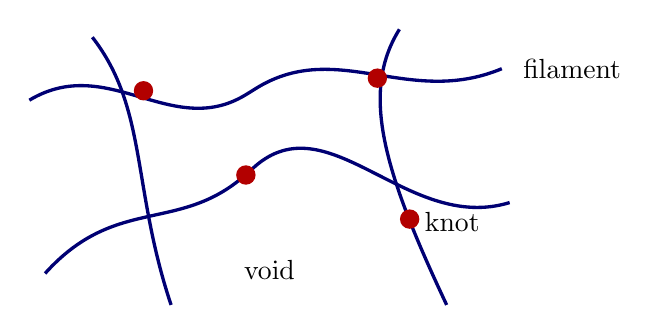
\begin{tikzpicture}[x=1cm,y=1cm]
  \draw[rounded corners=2pt,very thick,blue!45!black]
    (0.2,2.7) .. controls (1.2,3.3) and (2.0,2.2) .. (3.0,2.8)
    .. controls (4.1,3.5) and (5.0,2.6) .. (6.2,3.1);
  \draw[rounded corners=2pt,very thick,blue!45!black]
    (0.4,0.5) .. controls (1.3,1.5) and (2.1,1.0) .. (3.0,1.8)
    .. controls (4.0,2.7) and (5.0,1.0) .. (6.3,1.4);
  \draw[rounded corners=2pt,very thick,blue!45!black]
    (1.0,3.5) .. controls (1.7,2.6) and (1.5,1.6) .. (2.0,0.1);
  \draw[rounded corners=2pt,very thick,blue!45!black]
    (4.9,3.6) .. controls (4.4,2.8) and (4.7,1.8) .. (5.5,0.1);
  \fill[red!70!black] (1.65,2.82) circle (3.5pt);
  \fill[red!70!black] (4.62,2.98) circle (3.5pt);
  \fill[red!70!black] (2.95,1.75) circle (3.5pt);
  \fill[red!70!black] (5.03,1.19) circle (3.5pt);
  \node[align=center] at (3.25,0.55) {void};
  \node[right] at (6.35,3.1) {filament};
  \node[right] at (5.1,1.15) {knot};
\end{tikzpicture}\caption{Una analogía bidimensional clara de la red de cáusticas: las concentraciones lineales delimitan vacíos y convergen en nudos más brillantes. En tres dimensiones, los pliegues principales son láminas cuyas intersecciones forman filamentos y nodos.}\label{fig:c09-caustic-network}\end{figure}

Esta construcción sin fuerzas no sustituye a la teoría de perturbaciones cosmológicas. La gravedad es crucial para el crecimiento del contraste de densidad, la formación de halos y galaxias, y la estructura no lineal. El modelo simplificado aísla un hecho geométrico robusto: un flujo inicial con ligeras variaciones se pliega y se concentra de forma natural. También se podrían incluir pequeñas variaciones iniciales de densidad sin cambiar el argumento central basado en el jacobiano.

Así pues, hemos desplazado el misterio, pero no lo hemos eliminado. Introdujimos la inflación para estirar una región hasta hacerla extraordinariamente plana y uniforme. El cálculo de las cáusticas supone un campo inicial con pequeñas variaciones de velocidad. ¿De dónde surgió esa semilla inhomogénea? La siguiente lección trata las fluctuaciones cuánticas de los campos durante la inflación y pregunta cómo se convierten en las condiciones iniciales de la posterior red cósmica.

\section{Lo que se ha demostrado}

Un campo escalar homogéneo se comporta como una coordenada que se mueve en el potencial \(V(\phi)\). En una caja fija, obedece \(\ddot\phi=-V'(\phi)\). En una caja comóvil en expansión, el volumen físico \(a^3\) entra en la acción y da lugar a
\[
\ddot\phi+3H\dot\phi=-V'(\phi).
\]
La fricción de Hubble puede mantener al campo en un movimiento terminal lento sobre un potencial alto y poco profundo. Entonces su energía cinética se vuelve despreciable, su energía potencial mantiene \(H\) casi constante y \(a(t)\) crece aproximadamente de forma exponencial.

La expansión diluye los monopolos no deseados, suaviza la geometría e impulsa la curvatura hacia cero. Sin embargo, la inflación debe terminar. El campo abandona la meseta, oscila y transfiere su energía a las partículas calientes del recalentamiento. Quedan varias preguntas abiertas: la forma del potencial, la identidad y el estado inicial del inflatón, sus acoplamientos de recalentamiento y la diminuta energía del vacío que se observa hoy.

El éxito de la inflación plantea la pregunta final. Un universo perfectamente suavizado no contendría galaxias. El mapa de cáusticas
\[
y=x+v(x)t,
\qquad
\frac{dn}{dy}=\frac{1}{1+v'(x)t}
\]
muestra cómo pequeñas variaciones en un flujo inicial pueden generar láminas, filamentos y nudos pronunciados. No explica el origen de esas variaciones. El argumento pasa ahora a su origen cuántico.